\begin{frame}[fragile]{Visualização do algoritmo guloso para o problema do troco}

    \begin{figure}
        \centering

        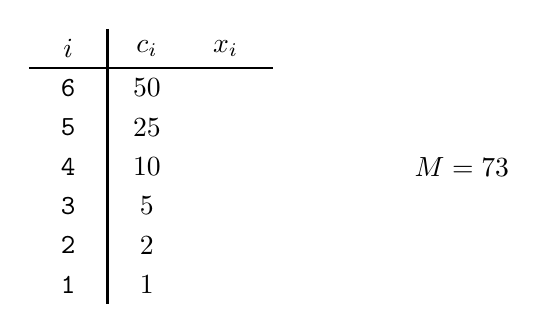
\begin{tikzpicture}
            \node at (5, 4) { $M = 73$ };

            \draw[thick] (-0.5, 5.25) -- (2.6, 5.25);
            \draw[thick] (0.5, 5.75) -- (0.5, 2.25);

            \node at (0, 5.5) { $i$ };
            \node at (0, 5) { \tt 6 };
            \node at (0, 4.5) { \tt 5 };
            \node at (0, 4) { \tt 4 };
            \node at (0, 3.5) { \tt 3 };
            \node at (0, 3) { \tt 2 };
            \node at (0, 2.5) { \tt 1 };

            \node at (1, 5.5) { $c_i$ };
            \node at (1, 5) { $50$ };
            \node at (1, 4.5) { $25$ };
            \node at (1, 4) { $10$ };
            \node at (1, 3.5) { $5$ };
            \node at (1, 3) { $2$ };
            \node at (1, 2.5) { $1$ };

            \node at (2, 5.5) { $x_i$ };
            %\node at (2, 5) { $50$ };
            %\node at (2, 4.5) { $25$ };
            %\node at (2, 4) { $10$ };
            %\node at (2, 3.5) { $5$ };
            %\node at (2, 3) { $2$ };
            %\node at (2, 2.5) { $1$ };


        \end{tikzpicture}

    \end{figure}

\end{frame}

\begin{frame}[fragile]{Visualização do algoritmo guloso para o problema do troco}

    \begin{figure}
        \centering

        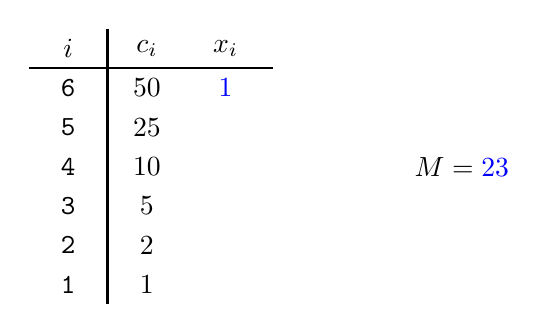
\begin{tikzpicture}
            \node at (5, 4) { $M = \textcolor{blue}{23}$ };

            \draw[thick] (-0.5, 5.25) -- (2.6, 5.25);
            \draw[thick] (0.5, 5.75) -- (0.5, 2.25);

            \node at (0, 5.5) { $i$ };
            \node at (0, 5) { \tt 6 };
            \node at (0, 4.5) { \tt 5 };
            \node at (0, 4) { \tt 4 };
            \node at (0, 3.5) { \tt 3 };
            \node at (0, 3) { \tt 2 };
            \node at (0, 2.5) { \tt 1 };

            \node at (1, 5.5) { $c_i$ };
            \node at (1, 5) { $50$ };
            \node at (1, 4.5) { $25$ };
            \node at (1, 4) { $10$ };
            \node at (1, 3.5) { $5$ };
            \node at (1, 3) { $2$ };
            \node at (1, 2.5) { $1$ };

            \node at (2, 5.5) { $x_i$ };
            \node at (2, 5) { \textcolor{blue}{$1$} };
            %\node at (2, 4.5) { $25$ };
            %\node at (2, 4) { $10$ };
            %\node at (2, 3.5) { $5$ };
            %\node at (2, 3) { $2$ };
            %\node at (2, 2.5) { $1$ };


        \end{tikzpicture}

    \end{figure}

\end{frame}

\begin{frame}[fragile]{Visualização do algoritmo guloso para o problema do troco}

    \begin{figure}
        \centering

        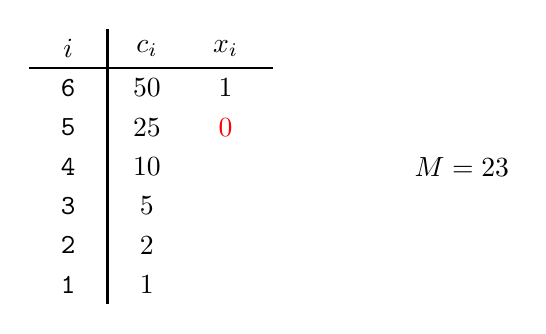
\begin{tikzpicture}
            \node at (5, 4) { $M = \textcolor{black}{23}$ };

            \draw[thick] (-0.5, 5.25) -- (2.6, 5.25);
            \draw[thick] (0.5, 5.75) -- (0.5, 2.25);

            \node at (0, 5.5) { $i$ };
            \node at (0, 5) { \tt 6 };
            \node at (0, 4.5) { \tt 5 };
            \node at (0, 4) { \tt 4 };
            \node at (0, 3.5) { \tt 3 };
            \node at (0, 3) { \tt 2 };
            \node at (0, 2.5) { \tt 1 };

            \node at (1, 5.5) { $c_i$ };
            \node at (1, 5) { $50$ };
            \node at (1, 4.5) { $25$ };
            \node at (1, 4) { $10$ };
            \node at (1, 3.5) { $5$ };
            \node at (1, 3) { $2$ };
            \node at (1, 2.5) { $1$ };

            \node at (2, 5.5) { $x_i$ };
            \node at (2, 5) { \textcolor{black}{$1$} };
            \node at (2, 4.5) { \textcolor{red}{$0$} };
            %\node at (2, 4) { $10$ };
            %\node at (2, 3.5) { $5$ };
            %\node at (2, 3) { $2$ };
            %\node at (2, 2.5) { $1$ };


        \end{tikzpicture}

    \end{figure}

\end{frame}

\begin{frame}[fragile]{Visualização do algoritmo guloso para o problema do troco}

    \begin{figure}
        \centering

        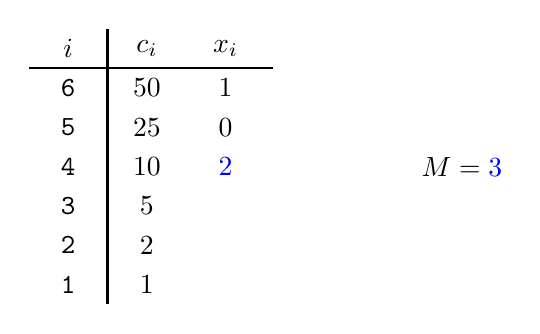
\begin{tikzpicture}
            \node at (5, 4) { $M = \textcolor{blue}{3}$ };

            \draw[thick] (-0.5, 5.25) -- (2.6, 5.25);
            \draw[thick] (0.5, 5.75) -- (0.5, 2.25);

            \node at (0, 5.5) { $i$ };
            \node at (0, 5) { \tt 6 };
            \node at (0, 4.5) { \tt 5 };
            \node at (0, 4) { \tt 4 };
            \node at (0, 3.5) { \tt 3 };
            \node at (0, 3) { \tt 2 };
            \node at (0, 2.5) { \tt 1 };

            \node at (1, 5.5) { $c_i$ };
            \node at (1, 5) { $50$ };
            \node at (1, 4.5) { $25$ };
            \node at (1, 4) { $10$ };
            \node at (1, 3.5) { $5$ };
            \node at (1, 3) { $2$ };
            \node at (1, 2.5) { $1$ };

            \node at (2, 5.5) { $x_i$ };
            \node at (2, 5) { \textcolor{black}{$1$} };
            \node at (2, 4.5) { \textcolor{black}{$0$} };
            \node at (2, 4) { \textcolor{blue}{$2$} };
            %\node at (2, 3.5) { $5$ };
            %\node at (2, 3) { $2$ };
            %\node at (2, 2.5) { $1$ };


        \end{tikzpicture}

    \end{figure}

\end{frame}

\begin{frame}[fragile]{Visualização do algoritmo guloso para o problema do troco}

    \begin{figure}
        \centering

        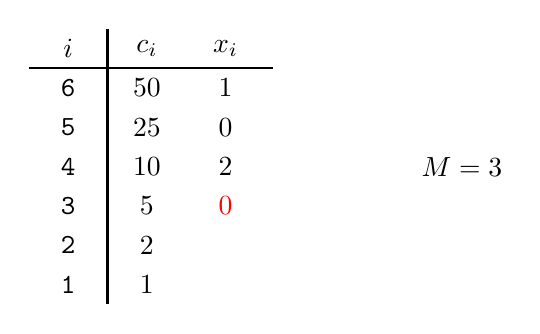
\begin{tikzpicture}
            \node at (5, 4) { $M = \textcolor{black}{3}$ };

            \draw[thick] (-0.5, 5.25) -- (2.6, 5.25);
            \draw[thick] (0.5, 5.75) -- (0.5, 2.25);

            \node at (0, 5.5) { $i$ };
            \node at (0, 5) { \tt 6 };
            \node at (0, 4.5) { \tt 5 };
            \node at (0, 4) { \tt 4 };
            \node at (0, 3.5) { \tt 3 };
            \node at (0, 3) { \tt 2 };
            \node at (0, 2.5) { \tt 1 };

            \node at (1, 5.5) { $c_i$ };
            \node at (1, 5) { $50$ };
            \node at (1, 4.5) { $25$ };
            \node at (1, 4) { $10$ };
            \node at (1, 3.5) { $5$ };
            \node at (1, 3) { $2$ };
            \node at (1, 2.5) { $1$ };

            \node at (2, 5.5) { $x_i$ };
            \node at (2, 5) { \textcolor{black}{$1$} };
            \node at (2, 4.5) { \textcolor{black}{$0$} };
            \node at (2, 4) { \textcolor{black}{$2$} };
            \node at (2, 3.5) { \textcolor{red}{$0$} };
            %\node at (2, 3) { $2$ };
            %\node at (2, 2.5) { $1$ };


        \end{tikzpicture}

    \end{figure}

\end{frame}

\begin{frame}[fragile]{Visualização do algoritmo guloso para o problema do troco}

    \begin{figure}
        \centering

        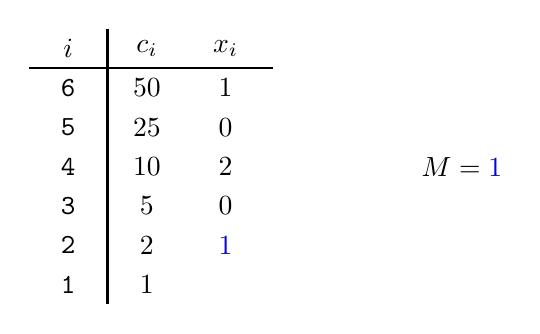
\begin{tikzpicture}
            \node at (5, 4) { $M = \textcolor{blue}{1}$ };

            \draw[thick] (-0.5, 5.25) -- (2.6, 5.25);
            \draw[thick] (0.5, 5.75) -- (0.5, 2.25);

            \node at (0, 5.5) { $i$ };
            \node at (0, 5) { \tt 6 };
            \node at (0, 4.5) { \tt 5 };
            \node at (0, 4) { \tt 4 };
            \node at (0, 3.5) { \tt 3 };
            \node at (0, 3) { \tt 2 };
            \node at (0, 2.5) { \tt 1 };

            \node at (1, 5.5) { $c_i$ };
            \node at (1, 5) { $50$ };
            \node at (1, 4.5) { $25$ };
            \node at (1, 4) { $10$ };
            \node at (1, 3.5) { $5$ };
            \node at (1, 3) { $2$ };
            \node at (1, 2.5) { $1$ };

            \node at (2, 5.5) { $x_i$ };
            \node at (2, 5) { \textcolor{black}{$1$} };
            \node at (2, 4.5) { \textcolor{black}{$0$} };
            \node at (2, 4) { \textcolor{black}{$2$} };
            \node at (2, 3.5) { \textcolor{black}{$0$} };
            \node at (2, 3) { \textcolor{blue}{$1$} };
            %\node at (2, 2.5) { $1$ };


        \end{tikzpicture}

    \end{figure}

\end{frame}

\begin{frame}[fragile]{Visualização do algoritmo guloso para o problema do troco}

    \begin{figure}
        \centering

        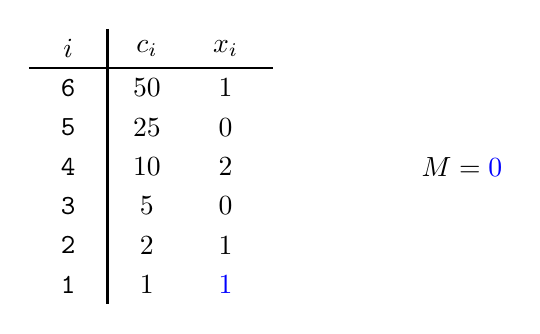
\begin{tikzpicture}
            \node at (5, 4) { $M = \textcolor{blue}{0}$ };

            \draw[thick] (-0.5, 5.25) -- (2.6, 5.25);
            \draw[thick] (0.5, 5.75) -- (0.5, 2.25);

            \node at (0, 5.5) { $i$ };
            \node at (0, 5) { \tt 6 };
            \node at (0, 4.5) { \tt 5 };
            \node at (0, 4) { \tt 4 };
            \node at (0, 3.5) { \tt 3 };
            \node at (0, 3) { \tt 2 };
            \node at (0, 2.5) { \tt 1 };

            \node at (1, 5.5) { $c_i$ };
            \node at (1, 5) { $50$ };
            \node at (1, 4.5) { $25$ };
            \node at (1, 4) { $10$ };
            \node at (1, 3.5) { $5$ };
            \node at (1, 3) { $2$ };
            \node at (1, 2.5) { $1$ };

            \node at (2, 5.5) { $x_i$ };
            \node at (2, 5) { \textcolor{black}{$1$} };
            \node at (2, 4.5) { \textcolor{black}{$0$} };
            \node at (2, 4) { \textcolor{black}{$2$} };
            \node at (2, 3.5) { \textcolor{black}{$0$} };
            \node at (2, 3) { \textcolor{black}{$1$} };
            \node at (2, 2.5) { \textcolor{blue}{$1$} };


        \end{tikzpicture}

    \end{figure}

\end{frame}
